%!TEX root = ../template.tex
%%%%%%%%%%%%%%%%%%%%%%%%%%%%%%%%%%%%%%%%%%%%%%%%%%%%%%%%%%%%%%%%%%%%
%% chapter4.tex
%% NOVA thesis document file
%%
%% Chapter with lots of dummy text
%%%%%%%%%%%%%%%%%%%%%%%%%%%%%%%%%%%%%%%%%%%%%%%%%%%%%%%%%%%%%%%%%%%%
\chapter{Elaboration Plan}
\label{cha:elaboration_plan}

This chapter presents the work plan for the elaboration phase of this dissertation. First we summarise the planned tasks as their planned time frames all gathered in a Gantt chart presented in section \ref{sec:workplan}. Then, in section \ref{sec:workplan_details} the taks are described in better detail and more in depth as well as referering the relevant related dependencies and risk-management options.

\section{Work Plan}
\label{sec:workplan}

\begin{figure}[htbp]
	\centerline{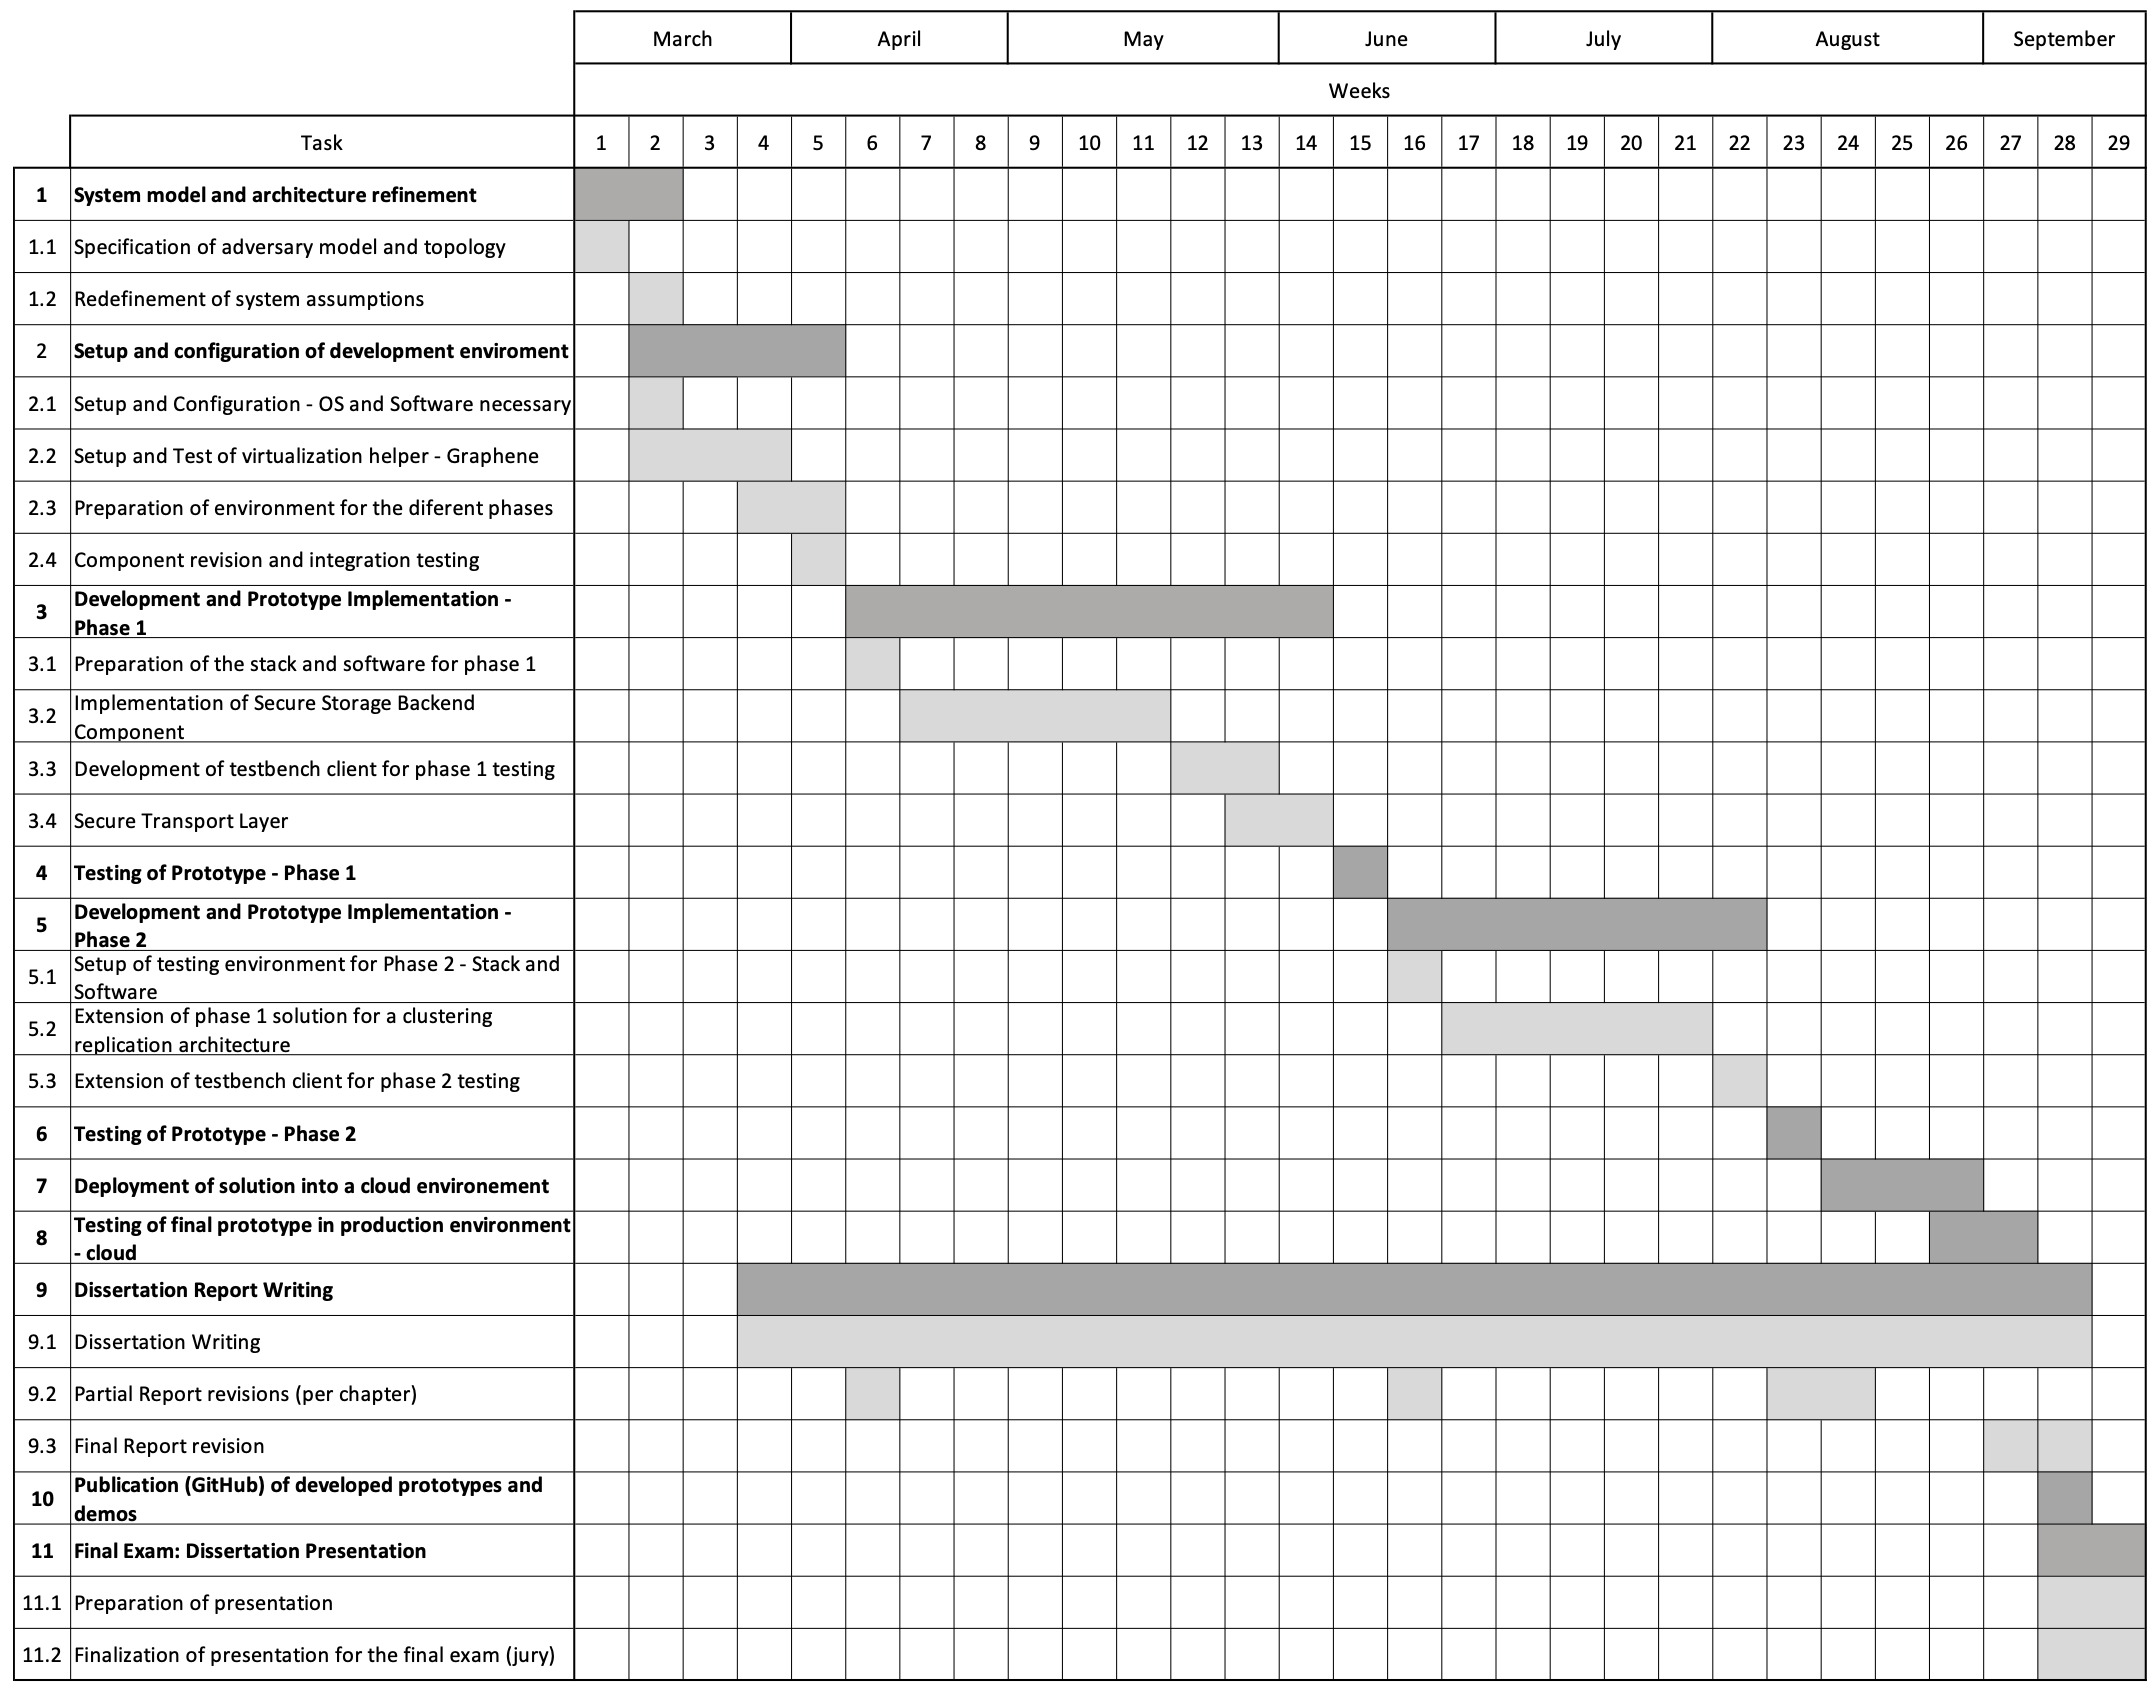
\includegraphics[angle=90, width=1.2\linewidth]{workplan}}%
	\label{fig:workplan}
	\caption{Work Plan}
\end{figure}

\section{Work Plan Detailed Tasks}
\label{sec:workplan_details}